\documentclass[letterpaper,twocolumn,10pt]{article}
\usepackage{epsfig,xspace,url}
\usepackage{authblk, cleveref}
\bibliographystyle{ieeetr}


\title{Course Project\\
Wii Write}
\author{Joshua Santos and Allan Howe}

\begin{document}

\maketitle

\subsection*{Introduction}
% Motivate and introduce the problem you are solving. Very briefly summarize your methodology, your experiments, and your important results.
The Nintendo Wii remote has been used in research as a cheap and common alternative to other accelerometers and inertial sensing, as discussed in~\cite{leeHacking}. The issue we are addressing is communication from one user to another via the Wii remote. This communication system could be used by people without fine motor skills for typing, or even the ability to talk.

We implement a Bluetooth connection between a Raspberry-Pi to a Wiimote. We design an ML model to detect letters drawn in the air which achieved 93\% accuracy on user dependent data. We experiment on the accuracy of the model and the Bluetooth packet loss at several distances. We find that the model is accurate enough to detect letters correctly and the Wiimote is capable of sending data up to 80ft without significant packet loss.

\subsection*{Related Work}
% Summarize the existing work related to your problem.
In previous work, the Wiimote has been reverse engineered and used in virtual reality~\cite{leeHacking} , physical activity tracking~\cite{Khan2013WiiActivity}, and even used to evaluate Parkinson's patients~\cite{SynnottWiiPD}. These works focused on using the Wiimote as an cheap alternative to other motion tracking devices.

There has been quite a bit of research in the area of air-writing. In~\cite{ChenAirWriting} they achieved a word error rate of 0.8\% with air-writing. The work in~\cite{YanayAirwriting} achieved 89.2\% accuracy on a letter prediction model that was user dependent, meaning the model was trained and tested on data from the same user.


\subsection*{Methodology}
% Describe your solution and any other methods you have used to solve your problem.
TODO: Josh, explain about how the Wiimote connection works? what tool are we using?

We used a Raspberry Pi Zero2W to connect to the Wiimote over Bluetooth. The Rasberry Pi receives raw accelerometer and button data from the Wiimote, and from this data predicts the drawn letter. To draw the letters, we hold the "A" button on the Wiimote and draw a stroke of the letter. Some letters like "H" have three strokes, while a letter like "S" only has one stroke. All leters we draw are upper-case. Accelerometer data is only sent while the "A" button is being held. Once the user is done writing a letter, the D-pad is pressed to indicate the end of letter.

We collected 25 samples of air-writing for every letter. For training, we used 80\% of this data, and the other 20\% was used for testing.

We tried several model architectures, and decided on a hybrid model that takes votes from two individual models. 

The first model is a random forest (RF) classifier, which takes extracted features from the accelerometer data to make a prediction. These features are: number of strokes, length of data, mean, standard deviation, minimum, maximum, for X, Y and Z data. The model builds 100 decision trees and combines their predictions for its output.

The second model is a multi-layer perceptron (MLP) that takes in the raw X, Y, Z data passes it through four fully connected hidden layers with sizes 256 $\rightarrow$ 128 $\rightarrow$ 64 $\rightarrow$ 32. Each layer uses ReLU activation and is trained using Adam optimizer with a learning rate of $1 \times 10^{-4}$. Since the MLP model input needs to have a standard size, we up-sample or down-sample to 100 samples for each axis input. 

Once the hybrid model was trained and at an acceptable accuracy, we implemented a full flow that allowed live data to be acquired, inference executed, and a letter predicted. We tested accuracy on live data, by air-writing each letter 10 times and evaluating against the model predictions.

Beyond building, training and testing a custom ML model, we also tested the range of the Wiimote with the Raspberry Pi setup. We tested the Wiimote at several distances in three related experiments. The first was testing the systems range while sending as many Bluetooth packets as we could in short period of time. We did this by holding the "A" button and shaking the Wiimote. This should send [TODO: X] number of packets per second and allowed us to compare with the actual number of packets received.

The second test was counting individual "A" button presses on the Wiimote, and seeing how many are missed by the Raspberry Pi at several distances.

The third test was running the full model inference pipeline for the same letter at different distances and observing how the accuracy changes. 


\subsection*{Implementation/Experimentation}
% Describe your experiments and your results. Discuss your results.
Individually, the two models were each about 90\% accurate, but when combine they reached 93-96\% on the test data. The reason for the range of accuracy, is because each time the MLP model was trained, it gave a different accuracy. TODO: what model accuracy did we end up saving in the .pkl?

The accuracy test on real world live data was 93.08\% accurate. In~\cref{fig:confusion_matrix} we show each letters true label and the model's prediction on the X axis from this live data test. We note here that the letter with the worst performance is "A". Oddly enough, it was confused here with "C" the most. 

TODO: Josh, explain results of the distance tests we did. packet number test, A button test, air-writing test.  


\begin{figure}[htb]
    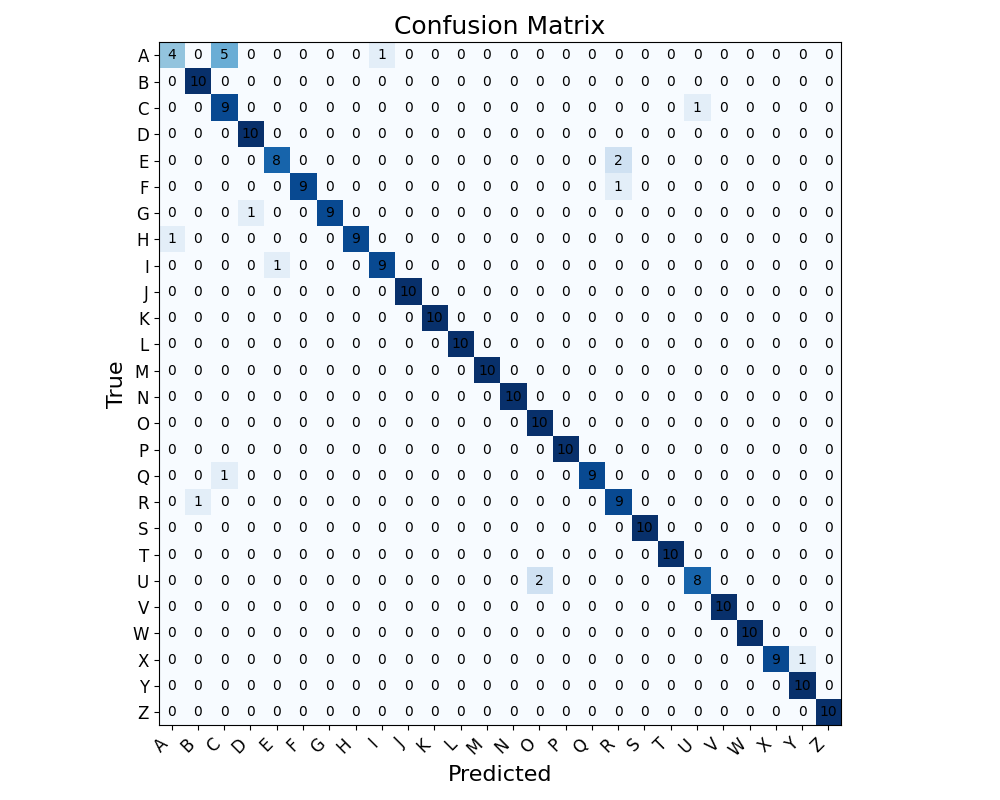
\includegraphics[width=\columnwidth]{../confusion_matrix.png}
    \caption{A confusion matrix showing the predicted labels vs the expected label for each letter}
    \label{fig:confusion_matrix}
\end{figure}
\subsection*{Conclusion}
% Summarize your work and your results. Indicated any future directions.
In this project, we implement a highly accurate air-writing ML model. We 

% List all the references you have used for this work.
\subsection*{References}
\renewcommand{\refname}{\vspace{-1.5em}}    % had to add this so bib does not add extra space or section header
\bibliography{references}


\end{document}
